Dans cette section nous allons présenter les différents artefacts Scrum que nous avions utilisé pour accomplir notre projet afin de nous faciliter la gestion des tâches. 
\subsection{Scrum board}
Le Scrum board est un outil visuel utilisé pour organiser et suivre les tâches dans chaque sprint (à faire, en cours, terminées). Il permet aux équipes de suivre l'avancement du travail tout au long des sprints. Sa mise à jour est la responsabilité des membres de l’équipe, facilitant la gestion des tâches et la visualisation de la progression\cite{Scrumboard}.

Nous avons utilisé l’outil \textbf{«OpenProject»} pour organiser les tâches sous forme de cartes réparties sur quatre colonnes : à faire, en cours, à tester et terminées. Cet outil nous a permis de suivre efficacement l'avancement de nos sprints, comme illustré dans la figure \ref{fig:boardOpenProject} représentant le Scrum board du Sprint 1.
\begin{figure}[H]
    \centering
    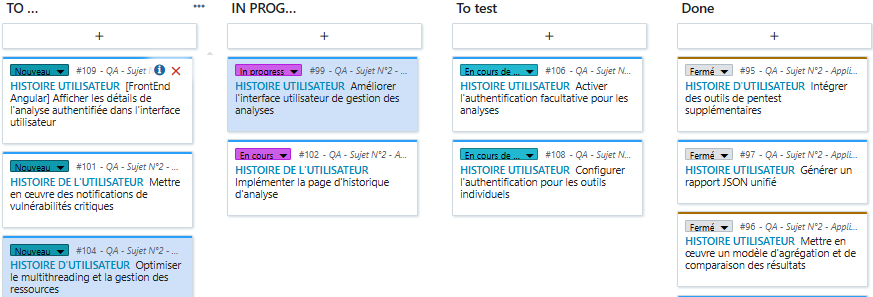
\includegraphics[width=\linewidth]{chapitres/ch2/img/board-sprit1.PNG}
    \caption{Scrum board Sprint 1}
    \label{fig:boardOpenProject}
\end{figure}
\vspace{-0.6cm}
\subsection{Burndown Chart}
Le Burndown Chart est un graphique visuel qui montre la quantité de travail terminée et celle restant à faire dans un sprint ou un projet, en fonction du temps écoulé. Il aide à estimer la capacité de l’équipe à atteindre ses objectifs dans les délais impartis et à détecter rapidement d’éventuelles dérives. La mise à jour régulière de ce graphique est essentielle pour anticiper les retards et ajuster le rythme de travail\cite{burndown}.

Nous avons généré les Burndown Charts à partir de l’avancement des tâches de chaque sprint. Ces graphiques nous ont permis de suivre efficacement notre progression et d’adapter notre charge de travail, comme illustré dans la figure \ref{fig:burndownChart} représentant le Burndown chart du projet.
\begin{figure}[H] 
    \centering 
    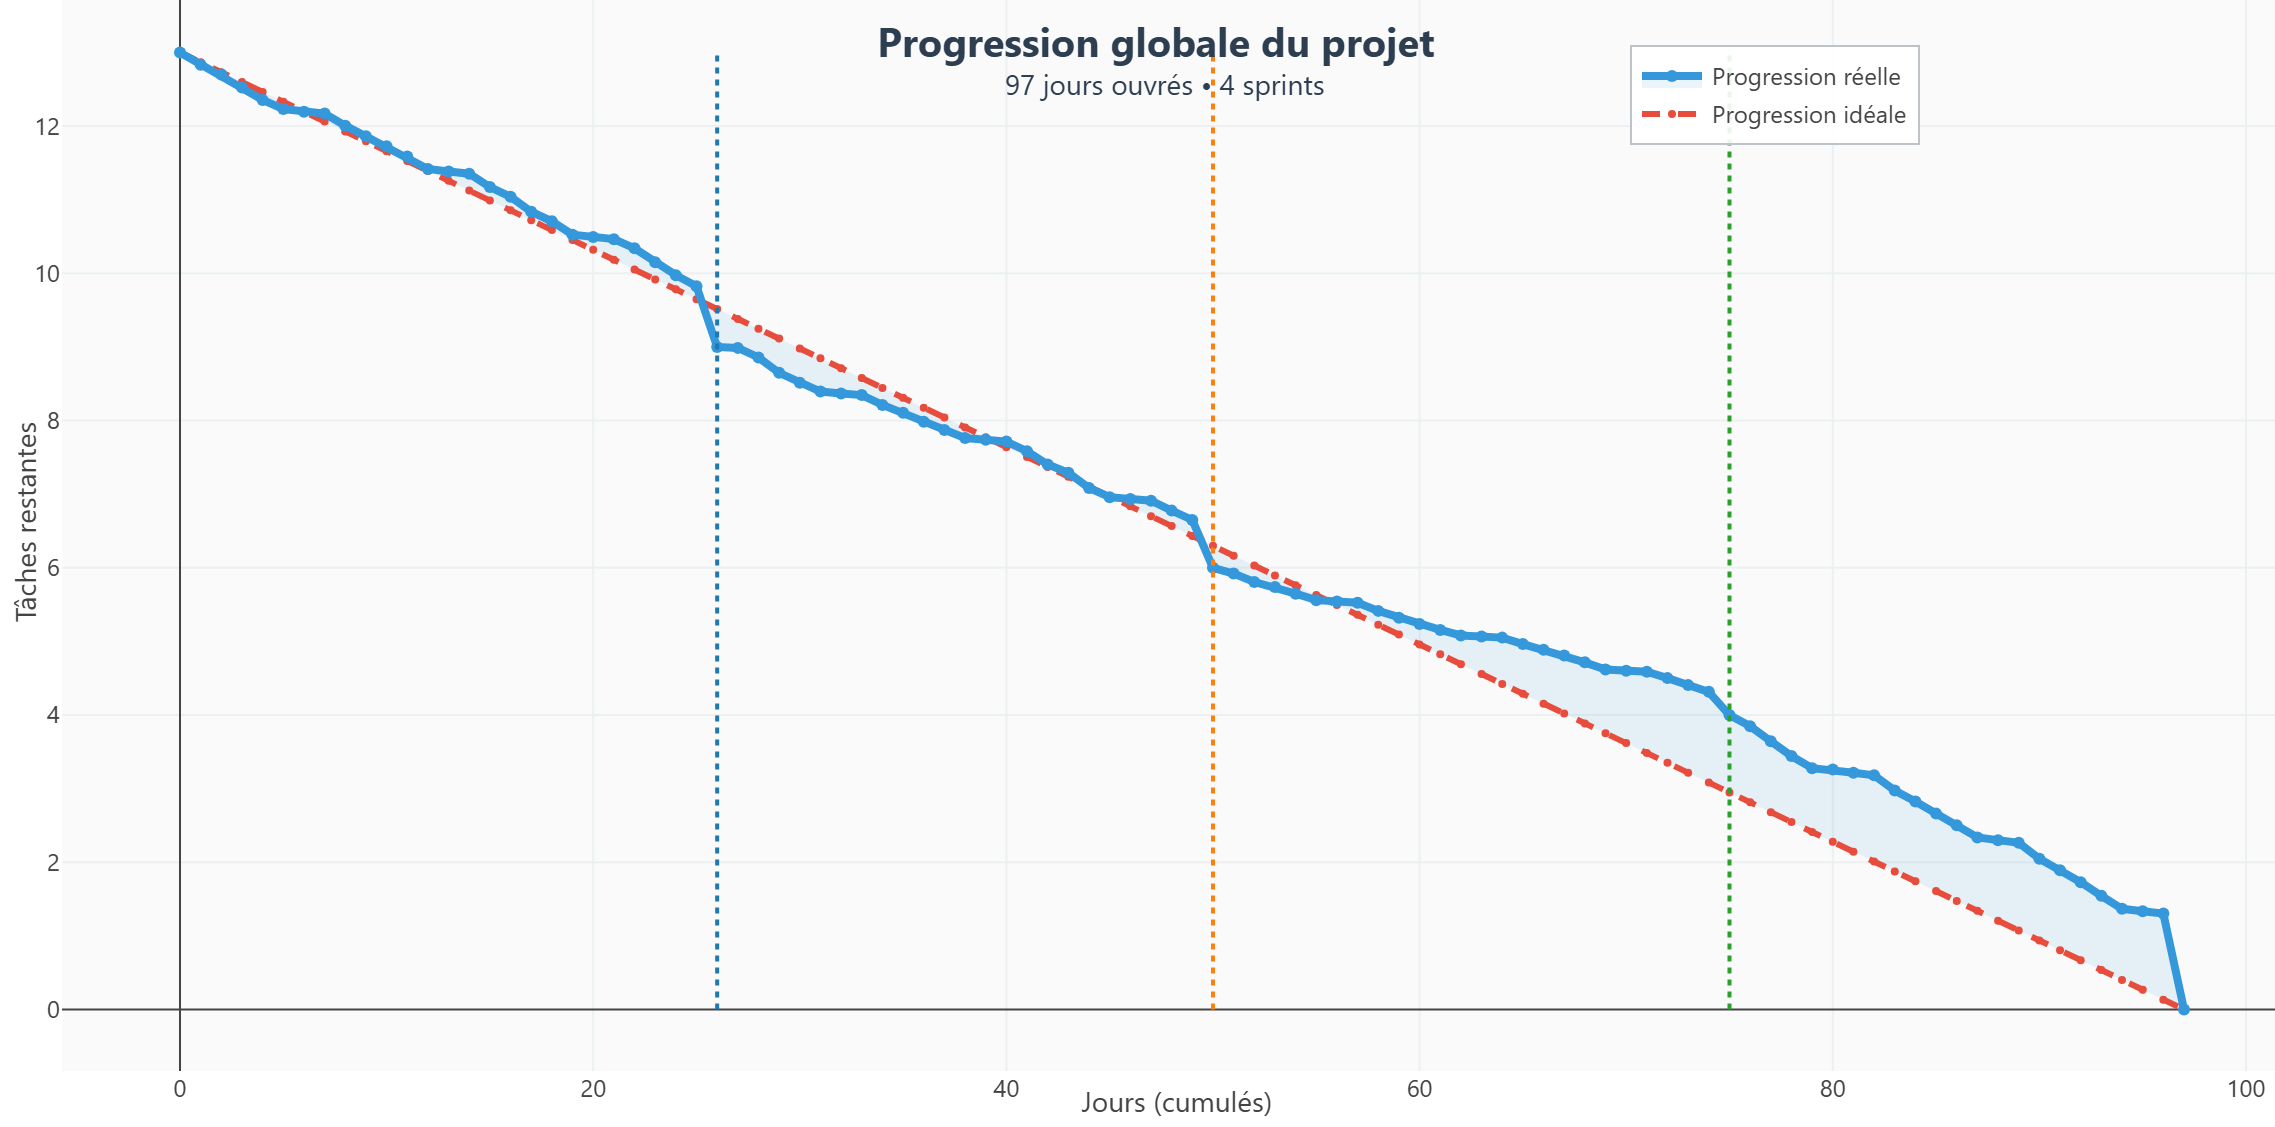
\includegraphics[width=0.97\linewidth]{chapitres/ch2/img/burndown.png} 
    \caption{Burndown chart projet} 
    \label{fig:burndownChart} \end{figure} 
\vspace{-0.8cm}
